\section{Analysis}
\ac{numerics} has to be a library regrouping other libraries. Each one corresponds to a part of the source of \ac{numerics} and is composed of source files in C or Fortran.\\
The architecture that suites is a set of directories to arrange all the libraries.\\
Into each directory according to a specific library, whereas programming languages are non object oriented, every file regroups functions relating to a particular kind of operation or system.


\section{Decomposition description}
The software components should be summarised. These components can be organised in various ways to provide the
views needed by the different members of the development team. The following views present the software
design.

\subsection{Decomposition view}
Here, we show the functional decomposition of the components. It consists in a list of components summarised~:
 
\begin{itemize}
		\item \ac{lapack}\\
		It is routines for solving systems of simultaneous linear equations, least-squares solutions of linear systems of equations, eigenvalue problems, and singular value problems.

        \item MP solver pack\\
		It regroups all the functionalities to solve non-smooth problems.
		
        \item \ac{ode} pack\\
		It is a collection of Fortran solvers for the initial value problem for ordinary differential equation systems.

        \item ...\\
\end{itemize}


\subsection{Dependency view}
Each module of \ac{numerics} is independent from the others. They make different kinds of computations and each module regroups specific low level functions.
However, \ac{lapack} is commonly used by the other "packs" (MP solver pack, \ac{ode} pack, \dots). It is the basis for the operations of these "packs".


\section{System architecture diagram with related description}
The figure \ref{fig: Tree view of the Numerics directories} represents the architecture of \ac{numerics}'s directories.
	\begin{figure}
	\begin{center}
	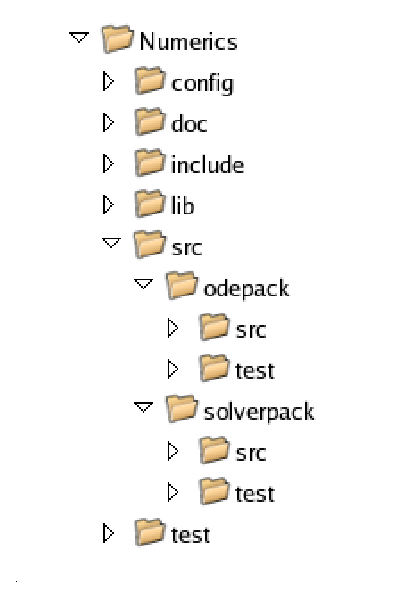
\includegraphics[scale=1.2, clip]{figure/NumericsDesign.eps}
	\caption{Tree view of the Numerics directories}
	\label{fig: Tree view of the Numerics directories}
	\end{center}
	\end{figure}
	
Each \textit{src} directory contains the source code of \ac{numerics}, especially \textit{src/odepack/src} and \textit{src/solverpack/src} which contain the code of \ac{ode} pack and MP solverpack.
